\documentclass[12pt,a4paper,fleqn]{article}
\usepackage[utf8]{inputenc}
\usepackage[russian]{babel}
\usepackage[shortcuts,cyremdash]{extdash}
\usepackage{wrapfig}
\usepackage{floatflt}
\usepackage{lipsum}
\usepackage{concmath}
\usepackage{euler}
\usepackage{libertine}
\usepackage{amsfonts}
\usepackage{amsmath}
\usepackage{hyperref}
\usepackage{graphicx}

\oddsidemargin=6mm

\parindent=0pt
\parskip=8pt
\pagestyle{empty}
\usepackage[normalem]{ulem} % uline
\usepackage{mdframed}
\usepackage{amsthm}
\theoremstyle{definition}
\newtheorem{Def}{Def.}
\newtheorem{Ex}{Ex.}

\newenvironment{Sol}[1][]{\textcolor{blue}{\bfseries Решение. }}{}

\flushbottom
\begin{document}Решим элементарную задачу на дифференцирование, которую автор данного учебника решал еще в 5 классе.


$\frac{cos( x  \cdot { 8 }^{{ x }^{ 4 }}) \cdot \log_{ 2.71828 }{cos( x ) +  2 }}{ 1  + sin( x )}
$

Мне было лень доказывать этот факт.

$( x )'_{x} =  1 $

(((Какой-то комментарий))) 

$(sin( x ))'_{x} = cos( x ) \cdot  1 $

Доказательство данного факта можно найти в \href{https://www.youtube.com/watch?v=dQw4w9WgXcQ}{видеолекции} 

$( 1 )'_{x} =  0 $

В результате простых рассуждений можно получить 

$( 1  + sin( x ))'_{x} =  0  + cos( x ) \cdot  1 $

(((Какой-то комментарий))) 

$( 2 )'_{x} =  0 $

Отсюда очевидно следует, что 

$( x )'_{x} =  1 $

Как рассказывали в начальной школе, 

$(cos( x ))'_{x} = ( -1  - sin( x )) \cdot  1 $

Используя Wolfram легко получить, что 

$(cos( x ) +  2 )'_{x} = ( -1  - sin( x )) \cdot  1  +  0 $

Доказательство будет дано в следующем издании учебника. 

$(\log_{ 2.71828 }{cos( x ) +  2 })'_{x} = \frac{( -1  - sin( x )) \cdot  1  +  0 }{\log_{ 2.71828 }{ 2.71828 } \cdot (cos( x ) +  2 )}
$

(((Какой-то комментарий))) 

$( x )'_{x} =  1 $

Легко видеть, что 

$({ x }^{ 4 })'_{x} =  4  \cdot  1  \cdot { x }^{ 4  -  1 }$

Используя Wolfram легко получить, что 

$({ 8 }^{{ x }^{ 4 }})'_{x} = \log_{ 2.71828 }{ 8 } \cdot  4  \cdot  1  \cdot { x }^{ 4  -  1 } \cdot { 8 }^{{ x }^{ 4 }}$

(((Какой-то комментарий))) 

$( x )'_{x} =  1 $

Доказательство будет дано в следующем издании учебника. 

$( x  \cdot { 8 }^{{ x }^{ 4 }})'_{x} =  1  \cdot { 8 }^{{ x }^{ 4 }} +  x  \cdot \log_{ 2.71828 }{ 8 } \cdot  4  \cdot  1  \cdot { x }^{ 4  -  1 } \cdot { 8 }^{{ x }^{ 4 }}$

Как рассказывали в начальной школе, 

$(cos( x  \cdot { 8 }^{{ x }^{ 4 }}))'_{x} = ( -1  - sin( x  \cdot { 8 }^{{ x }^{ 4 }})) \cdot ( 1  \cdot { 8 }^{{ x }^{ 4 }} +  x  \cdot \log_{ 2.71828 }{ 8 } \cdot  4  \cdot  1  \cdot { x }^{ 4  -  1 } \cdot { 8 }^{{ x }^{ 4 }})$

Тут могла быть Ваша реклама. 

$(cos( x  \cdot { 8 }^{{ x }^{ 4 }}) \cdot \log_{ 2.71828 }{cos( x ) +  2 })'_{x} = ( -1  - sin( x  \cdot { 8 }^{{ x }^{ 4 }})) \cdot ( 1  \cdot { 8 }^{{ x }^{ 4 }} +  x  \cdot \log_{ 2.71828 }{ 8 } \cdot  4  \cdot  1  \cdot { x }^{ 4  -  1 } \cdot { 8 }^{{ x }^{ 4 }}) \cdot \log_{ 2.71828 }{cos( x ) +  2 } + cos( x  \cdot { 8 }^{{ x }^{ 4 }}) \cdot \frac{( -1  - sin( x )) \cdot  1  +  0 }{\log_{ 2.71828 }{ 2.71828 } \cdot (cos( x ) +  2 )}
$

В любом учебнике написано, что 

$(\frac{cos( x  \cdot { 8 }^{{ x }^{ 4 }}) \cdot \log_{ 2.71828 }{cos( x ) +  2 }}{ 1  + sin( x )}
)'_{x} = \frac{(( -1  - sin( x  \cdot { 8 }^{{ x }^{ 4 }})) \cdot ( 1  \cdot { 8 }^{{ x }^{ 4 }} +  x  \cdot \log_{ 2.71828 }{ 8 } \cdot  4  \cdot  1  \cdot { x }^{ 4  -  1 } \cdot { 8 }^{{ x }^{ 4 }}) \cdot \log_{ 2.71828 }{cos( x ) +  2 } + cos( x  \cdot { 8 }^{{ x }^{ 4 }}) \cdot \frac{( -1  - sin( x )) \cdot  1  +  0 }{\log_{ 2.71828 }{ 2.71828 } \cdot (cos( x ) +  2 )}
) \cdot ( 1  + sin( x )) - cos( x  \cdot { 8 }^{{ x }^{ 4 }}) \cdot \log_{ 2.71828 }{cos( x ) +  2 } \cdot ( 0  + cos( x ) \cdot  1 )}{( 1  + sin( x )) \cdot ( 1  + sin( x ))}
$
 1 $

Доказательство будет дано в следующем издании учебника. 

$ 4  \cdot  1  =  4 $

Отсюда очевидно следует, что 

$ 4  -  1  =  3 $

Примем без доказательства, что 

${ x }^{ 3 } = { x }^{ 3 }$

Легко видеть, что 

$ 4  \cdot { x }^{ 3 } =  4  \cdot { x }^{ 3 }$

Легко видеть, что 

$ 1  \cdot  4  \cdot { x }^{ 3 } =  1  \cdot  4  \cdot { x }^{ 3 }$

Зачем Вы читаете эти комментарии, в них нет никакого смысла... 

${ x }^{ 4 } = { x }^{ 4 }$

Очевидно, что 

${ 8 }^{{ x }^{ 4 }} = { 8 }^{{ x }^{ 4 }}$

Нетрудно догадаться, что 

$ 1  \cdot  4  \cdot { x }^{ 3 } \cdot { 8 }^{{ x }^{ 4 }} =  1  \cdot  4  \cdot { x }^{ 3 } \cdot { 8 }^{{ x }^{ 4 }}$

Используя Wolfram легко получить, что 

$ x  \cdot  1  \cdot  4  \cdot { x }^{ 3 } \cdot { 8 }^{{ x }^{ 4 }} =  x  \cdot  1  \cdot  4  \cdot { x }^{ 3 } \cdot { 8 }^{{ x }^{ 4 }}$

В любом учебнике написано, что 

$ 1  \cdot { 8 }^{{ x }^{ 4 }} +  x  \cdot  1  \cdot  4  \cdot { x }^{ 3 } \cdot { 8 }^{{ x }^{ 4 }} =  1  \cdot { 8 }^{{ x }^{ 4 }} +  x  \cdot  1  \cdot  4  \cdot { x }^{ 3 } \cdot { 8 }^{{ x }^{ 4 }}$

Используя теорему 1000 из тома 7 главы 666 и лемму 42 из тома 13 главы 66 нетрудно получить, что 

$( -1  - sin( x  \cdot { 8 }^{{ x }^{ 4 }})) \cdot ( 1  \cdot { 8 }^{{ x }^{ 4 }} +  x  \cdot  1  \cdot  4  \cdot { x }^{ 3 } \cdot { 8 }^{{ x }^{ 4 }}) = ( -1  - sin( x  \cdot { 8 }^{{ x }^{ 4 }})) \cdot ( 1  \cdot { 8 }^{{ x }^{ 4 }} +  x  \cdot  1  \cdot  4  \cdot { x }^{ 3 } \cdot { 8 }^{{ x }^{ 4 }})$

Оставим доказательство данного факта читателю в качестве несложного упражнения. 

$cos( x ) +  2  = cos( x ) +  2 $

Используя теорему 1000 из тома 7 главы 666 и лемму 42 из тома 13 главы 66 нетрудно получить, что 

$\log_{ 2.71828 }{cos( x ) +  2 } = \log_{ 2.71828 }{cos( x ) +  2 }$

Примем без доказательства, что 

$( -1  - sin( x  \cdot { 8 }^{{ x }^{ 4 }})) \cdot ( 1  \cdot { 8 }^{{ x }^{ 4 }} +  x  \cdot  1  \cdot  4  \cdot { x }^{ 3 } \cdot { 8 }^{{ x }^{ 4 }}) \cdot \log_{ 2.71828 }{cos( x ) +  2 } = ( -1  - sin( x  \cdot { 8 }^{{ x }^{ 4 }})) \cdot ( 1  \cdot { 8 }^{{ x }^{ 4 }} +  x  \cdot  1  \cdot  4  \cdot { x }^{ 3 } \cdot { 8 }^{{ x }^{ 4 }}) \cdot \log_{ 2.71828 }{cos( x ) +  2 }$

(((Какой-то комментарий))) 

${ x }^{ 4 } = { x }^{ 4 }$

Используя теорему 1000 из тома 7 главы 666 и лемму 42 из тома 13 главы 66 нетрудно получить, что 

${ 8 }^{{ x }^{ 4 }} = { 8 }^{{ x }^{ 4 }}$

Как рассказывали в начальной школе, 

$ x  \cdot { 8 }^{{ x }^{ 4 }} =  x  \cdot { 8 }^{{ x }^{ 4 }}$

В результате простых рассуждений можно получить 

$sin( x ) = sin( x )$

Как рассказывали в начальной школе, 

$ -1  - sin( x ) =  -1  - sin( x )$

Мне было лень доказывать этот факт.

$( -1  - sin( x )) \cdot  1  = ( -1  - sin( x )) \cdot  1 $

Отсюда очевидно следует, что 

$( -1  - sin( x )) \cdot  1  +  0  = ( -1  - sin( x )) \cdot  1  +  0 $

Как рассказывали в начальной школе, 

$\log_{ 2.71828 }{ 2.71828 } =  1 $

В результате простых рассуждений можно получить 

$cos( x ) +  2  = cos( x ) +  2 $

Нетрудно догадаться, что 

$ 1  \cdot (cos( x ) +  2 ) =  1  \cdot (cos( x ) +  2 )$

Используя Wolfram легко получить, что 

$\frac{( -1  - sin( x )) \cdot  1  +  0 }{ 1  \cdot (cos( x ) +  2 )}
 = \frac{( -1  - sin( x )) \cdot  1  +  0 }{ 1  \cdot (cos( x ) +  2 )}
$

Отсюда очевидно следует, что 

$cos( x  \cdot { 8 }^{{ x }^{ 4 }}) \cdot \frac{( -1  - sin( x )) \cdot  1  +  0 }{ 1  \cdot (cos( x ) +  2 )}
 = cos( x  \cdot { 8 }^{{ x }^{ 4 }}) \cdot \frac{( -1  - sin( x )) \cdot  1  +  0 }{ 1  \cdot (cos( x ) +  2 )}
$

Применяя знания, полученные на прошлой лекции, читатель без труда получит, что 

$( -1  - sin( x  \cdot { 8 }^{{ x }^{ 4 }})) \cdot ( 1  \cdot { 8 }^{{ x }^{ 4 }} +  x  \cdot  1  \cdot  4  \cdot { x }^{ 3 } \cdot { 8 }^{{ x }^{ 4 }}) \cdot \log_{ 2.71828 }{cos( x ) +  2 } + cos( x  \cdot { 8 }^{{ x }^{ 4 }}) \cdot \frac{( -1  - sin( x )) \cdot  1  +  0 }{ 1  \cdot (cos( x ) +  2 )}
 = ( -1  - sin( x  \cdot { 8 }^{{ x }^{ 4 }})) \cdot ( 1  \cdot { 8 }^{{ x }^{ 4 }} +  x  \cdot  1  \cdot  4  \cdot { x }^{ 3 } \cdot { 8 }^{{ x }^{ 4 }}) \cdot \log_{ 2.71828 }{cos( x ) +  2 } + cos( x  \cdot { 8 }^{{ x }^{ 4 }}) \cdot \frac{( -1  - sin( x )) \cdot  1  +  0 }{ 1  \cdot (cos( x ) +  2 )}
$

Зачем Вы читаете эти комментарии, в них нет никакого смысла... 

$ 1  + sin( x ) =  1  + sin( x )$

Мне было лень доказывать этот факт.

$(( -1  - sin( x  \cdot { 8 }^{{ x }^{ 4 }})) \cdot ( 1  \cdot { 8 }^{{ x }^{ 4 }} +  x  \cdot  1  \cdot  4  \cdot { x }^{ 3 } \cdot { 8 }^{{ x }^{ 4 }}) \cdot \log_{ 2.71828 }{cos( x ) +  2 } + cos( x  \cdot { 8 }^{{ x }^{ 4 }}) \cdot \frac{( -1  - sin( x )) \cdot  1  +  0 }{ 1  \cdot (cos( x ) +  2 )}
) \cdot ( 1  + sin( x )) = (( -1  - sin( x  \cdot { 8 }^{{ x }^{ 4 }})) \cdot ( 1  \cdot { 8 }^{{ x }^{ 4 }} +  x  \cdot  1  \cdot  4  \cdot { x }^{ 3 } \cdot { 8 }^{{ x }^{ 4 }}) \cdot \log_{ 2.71828 }{cos( x ) +  2 } + cos( x  \cdot { 8 }^{{ x }^{ 4 }}) \cdot \frac{( -1  - sin( x )) \cdot  1  +  0 }{ 1  \cdot (cos( x ) +  2 )}
) \cdot ( 1  + sin( x ))$

Как рассказывали в начальной школе, 

${ x }^{ 4 } = { x }^{ 4 }$

Тут могла быть Ваша реклама. 

${ 8 }^{{ x }^{ 4 }} = { 8 }^{{ x }^{ 4 }}$

В результате простых рассуждений можно получить 

$ x  \cdot { 8 }^{{ x }^{ 4 }} =  x  \cdot { 8 }^{{ x }^{ 4 }}$

Доказательство данного факта можно найти в \href{https://www.youtube.com/watch?v=dQw4w9WgXcQ}{видеолекции} 

$cos( x ) +  2  = cos( x ) +  2 $

Нетрудно догадаться, что 

$\log_{ 2.71828 }{cos( x ) +  2 } = \log_{ 2.71828 }{cos( x ) +  2 }$

В результате простых рассуждений можно получить 

$cos( x  \cdot { 8 }^{{ x }^{ 4 }}) \cdot \log_{ 2.71828 }{cos( x ) +  2 } = cos( x  \cdot { 8 }^{{ x }^{ 4 }}) \cdot \log_{ 2.71828 }{cos( x ) +  2 }$

Доказательство данного факта можно найти в \href{https://www.youtube.com/watch?v=dQw4w9WgXcQ}{видеолекции} 

$cos( x ) = cos( x )$

Оставим доказательство данного факта читателю в качестве несложного упражнения. 

$cos( x ) \cdot  1  = cos( x ) \cdot  1 $

В результате простых рассуждений можно получить 

$ 0  + cos( x ) \cdot  1  =  0  + cos( x ) \cdot  1 $

Очевидно, что 

$cos( x  \cdot { 8 }^{{ x }^{ 4 }}) \cdot \log_{ 2.71828 }{cos( x ) +  2 } \cdot ( 0  + cos( x ) \cdot  1 ) = cos( x  \cdot { 8 }^{{ x }^{ 4 }}) \cdot \log_{ 2.71828 }{cos( x ) +  2 } \cdot ( 0  + cos( x ) \cdot  1 )$

Оставим доказательство данного факта читателю в качестве несложного упражнения. 

$(( -1  - sin( x  \cdot { 8 }^{{ x }^{ 4 }})) \cdot ( 1  \cdot { 8 }^{{ x }^{ 4 }} +  x  \cdot  1  \cdot  4  \cdot { x }^{ 3 } \cdot { 8 }^{{ x }^{ 4 }}) \cdot \log_{ 2.71828 }{cos( x ) +  2 } + cos( x  \cdot { 8 }^{{ x }^{ 4 }}) \cdot \frac{( -1  - sin( x )) \cdot  1  +  0 }{ 1  \cdot (cos( x ) +  2 )}
) \cdot ( 1  + sin( x )) - cos( x  \cdot { 8 }^{{ x }^{ 4 }}) \cdot \log_{ 2.71828 }{cos( x ) +  2 } \cdot ( 0  + cos( x ) \cdot  1 ) = (( -1  - sin( x  \cdot { 8 }^{{ x }^{ 4 }})) \cdot ( 1  \cdot { 8 }^{{ x }^{ 4 }} +  x  \cdot  1  \cdot  4  \cdot { x }^{ 3 } \cdot { 8 }^{{ x }^{ 4 }}) \cdot \log_{ 2.71828 }{cos( x ) +  2 } + cos( x  \cdot { 8 }^{{ x }^{ 4 }}) \cdot \frac{( -1  - sin( x )) \cdot  1  +  0 }{ 1  \cdot (cos( x ) +  2 )}
) \cdot ( 1  + sin( x )) - cos( x  \cdot { 8 }^{{ x }^{ 4 }}) \cdot \log_{ 2.71828 }{cos( x ) +  2 } \cdot ( 0  + cos( x ) \cdot  1 )$

Примем без доказательства, что 

$ 1  + sin( x ) =  1  + sin( x )$

В результате простых рассуждений можно получить 

$ 1  + sin( x ) =  1  + sin( x )$

В результате простых рассуждений можно получить 

$( 1  + sin( x )) \cdot ( 1  + sin( x )) = ( 1  + sin( x )) \cdot ( 1  + sin( x ))$

Очевидно, что 

$\frac{(( -1  - sin( x  \cdot { 8 }^{{ x }^{ 4 }})) \cdot ( 1  \cdot { 8 }^{{ x }^{ 4 }} +  x  \cdot  1  \cdot  4  \cdot { x }^{ 3 } \cdot { 8 }^{{ x }^{ 4 }}) \cdot \log_{ 2.71828 }{cos( x ) +  2 } + cos( x  \cdot { 8 }^{{ x }^{ 4 }}) \cdot \frac{( -1  - sin( x )) \cdot  1  +  0 }{ 1  \cdot (cos( x ) +  2 )}
) \cdot ( 1  + sin( x )) - cos( x  \cdot { 8 }^{{ x }^{ 4 }}) \cdot \log_{ 2.71828 }{cos( x ) +  2 } \cdot ( 0  + cos( x ) \cdot  1 )}{( 1  + sin( x )) \cdot ( 1  + sin( x ))}
 = \frac{(( -1  - sin( x  \cdot { 8 }^{{ x }^{ 4 }})) \cdot ( 1  \cdot { 8 }^{{ x }^{ 4 }} +  x  \cdot  1  \cdot  4  \cdot { x }^{ 3 } \cdot { 8 }^{{ x }^{ 4 }}) \cdot \log_{ 2.71828 }{cos( x ) +  2 } + cos( x  \cdot { 8 }^{{ x }^{ 4 }}) \cdot \frac{( -1  - sin( x )) \cdot  1  +  0 }{ 1  \cdot (cos( x ) +  2 )}
) \cdot ( 1  + sin( x )) - cos( x  \cdot { 8 }^{{ x }^{ 4 }}) \cdot \log_{ 2.71828 }{cos( x ) +  2 } \cdot ( 0  + cos( x ) \cdot  1 )}{( 1  + sin( x )) \cdot ( 1  + sin( x ))}
$
{ 8 }^{{ x }^{ 4 }}$

Легко видеть, что 

${ x }^{ 3 } = { x }^{ 3 }$

Используя теорему 1000 из тома 7 главы 666 и лемму 42 из тома 13 главы 66 нетрудно получить, что 

$ 4  \cdot { x }^{ 3 } =  4  \cdot { x }^{ 3 }$

Применяя знания, полученные на прошлой лекции, читатель без труда получит, что 

$ 1  \cdot  4  \cdot { x }^{ 3 } =  4  \cdot { x }^{ 3 }$

Используя Wolfram легко получить, что 

${ x }^{ 4 } = { x }^{ 4 }$

Доказательство будет дано в следующем издании учебника. 

${ 8 }^{{ x }^{ 4 }} = { 8 }^{{ x }^{ 4 }}$

В результате простых рассуждений можно получить 

$ 4  \cdot { x }^{ 3 } \cdot { 8 }^{{ x }^{ 4 }} =  4  \cdot { x }^{ 3 } \cdot { 8 }^{{ x }^{ 4 }}$

Тут могла быть Ваша реклама. 

$ x  \cdot  4  \cdot { x }^{ 3 } \cdot { 8 }^{{ x }^{ 4 }} =  x  \cdot  4  \cdot { x }^{ 3 } \cdot { 8 }^{{ x }^{ 4 }}$

В любом учебнике написано, что 

${ 8 }^{{ x }^{ 4 }} +  x  \cdot  4  \cdot { x }^{ 3 } \cdot { 8 }^{{ x }^{ 4 }} = { 8 }^{{ x }^{ 4 }} +  x  \cdot  4  \cdot { x }^{ 3 } \cdot { 8 }^{{ x }^{ 4 }}$

Доказательство данного факта можно найти в \href{https://www.youtube.com/watch?v=dQw4w9WgXcQ}{видеолекции} 

$( -1  - sin( x  \cdot { 8 }^{{ x }^{ 4 }})) \cdot ({ 8 }^{{ x }^{ 4 }} +  x  \cdot  4  \cdot { x }^{ 3 } \cdot { 8 }^{{ x }^{ 4 }}) = ( -1  - sin( x  \cdot { 8 }^{{ x }^{ 4 }})) \cdot ({ 8 }^{{ x }^{ 4 }} +  x  \cdot  4  \cdot { x }^{ 3 } \cdot { 8 }^{{ x }^{ 4 }})$

Как рассказывали в начальной школе, 

$cos( x ) +  2  = cos( x ) +  2 $

Доказательство данного факта можно найти в \href{https://www.youtube.com/watch?v=dQw4w9WgXcQ}{видеолекции} 

$\log_{ 2.71828 }{cos( x ) +  2 } = \log_{ 2.71828 }{cos( x ) +  2 }$

Доказательство данного факта можно найти в \href{https://www.youtube.com/watch?v=dQw4w9WgXcQ}{видеолекции} 

$( -1  - sin( x  \cdot { 8 }^{{ x }^{ 4 }})) \cdot ({ 8 }^{{ x }^{ 4 }} +  x  \cdot  4  \cdot { x }^{ 3 } \cdot { 8 }^{{ x }^{ 4 }}) \cdot \log_{ 2.71828 }{cos( x ) +  2 } = ( -1  - sin( x  \cdot { 8 }^{{ x }^{ 4 }})) \cdot ({ 8 }^{{ x }^{ 4 }} +  x  \cdot  4  \cdot { x }^{ 3 } \cdot { 8 }^{{ x }^{ 4 }}) \cdot \log_{ 2.71828 }{cos( x ) +  2 }$

Мне было лень доказывать этот факт.

${ x }^{ 4 } = { x }^{ 4 }$

Тут могла быть Ваша реклама. 

${ 8 }^{{ x }^{ 4 }} = { 8 }^{{ x }^{ 4 }}$

Используя теорему 1000 из тома 7 главы 666 и лемму 42 из тома 13 главы 66 нетрудно получить, что 

$ x  \cdot { 8 }^{{ x }^{ 4 }} =  x  \cdot { 8 }^{{ x }^{ 4 }}$

Нетрудно догадаться, что 

$sin( x ) = sin( x )$

Легко видеть, что 

$ -1  - sin( x ) =  -1  - sin( x )$

Применяя знания, полученные на прошлой лекции, читатель без труда получит, что 

$( -1  - sin( x )) \cdot  1  =  -1  - sin( x )$

(((Какой-то комментарий))) 

$ -1  - sin( x ) +  0  =  -1  - sin( x )$

Доказательство данного факта можно найти в \href{https://www.youtube.com/watch?v=dQw4w9WgXcQ}{видеолекции} 

$cos( x ) +  2  = cos( x ) +  2 $

Доказательство будет дано в следующем издании учебника. 

$ 1  \cdot (cos( x ) +  2 ) = cos( x ) +  2 $

Оставим доказательство данного факта читателю в качестве несложного упражнения. 

$\frac{ -1  - sin( x )}{cos( x ) +  2 }
 = \frac{ -1  - sin( x )}{cos( x ) +  2 }
$

Применяя знания, полученные на прошлой лекции, читатель без труда получит, что 

$cos( x  \cdot { 8 }^{{ x }^{ 4 }}) \cdot \frac{ -1  - sin( x )}{cos( x ) +  2 }
 = cos( x  \cdot { 8 }^{{ x }^{ 4 }}) \cdot \frac{ -1  - sin( x )}{cos( x ) +  2 }
$

Тут могла быть Ваша реклама. 

$( -1  - sin( x  \cdot { 8 }^{{ x }^{ 4 }})) \cdot ({ 8 }^{{ x }^{ 4 }} +  x  \cdot  4  \cdot { x }^{ 3 } \cdot { 8 }^{{ x }^{ 4 }}) \cdot \log_{ 2.71828 }{cos( x ) +  2 } + cos( x  \cdot { 8 }^{{ x }^{ 4 }}) \cdot \frac{ -1  - sin( x )}{cos( x ) +  2 }
 = ( -1  - sin( x  \cdot { 8 }^{{ x }^{ 4 }})) \cdot ({ 8 }^{{ x }^{ 4 }} +  x  \cdot  4  \cdot { x }^{ 3 } \cdot { 8 }^{{ x }^{ 4 }}) \cdot \log_{ 2.71828 }{cos( x ) +  2 } + cos( x  \cdot { 8 }^{{ x }^{ 4 }}) \cdot \frac{ -1  - sin( x )}{cos( x ) +  2 }
$

Доказательство будет дано в следующем издании учебника. 

$ 1  + sin( x ) =  1  + sin( x )$

Используя теорему 1000 из тома 7 главы 666 и лемму 42 из тома 13 главы 66 нетрудно получить, что 

$(( -1  - sin( x  \cdot { 8 }^{{ x }^{ 4 }})) \cdot ({ 8 }^{{ x }^{ 4 }} +  x  \cdot  4  \cdot { x }^{ 3 } \cdot { 8 }^{{ x }^{ 4 }}) \cdot \log_{ 2.71828 }{cos( x ) +  2 } + cos( x  \cdot { 8 }^{{ x }^{ 4 }}) \cdot \frac{ -1  - sin( x )}{cos( x ) +  2 }
) \cdot ( 1  + sin( x )) = (( -1  - sin( x  \cdot { 8 }^{{ x }^{ 4 }})) \cdot ({ 8 }^{{ x }^{ 4 }} +  x  \cdot  4  \cdot { x }^{ 3 } \cdot { 8 }^{{ x }^{ 4 }}) \cdot \log_{ 2.71828 }{cos( x ) +  2 } + cos( x  \cdot { 8 }^{{ x }^{ 4 }}) \cdot \frac{ -1  - sin( x )}{cos( x ) +  2 }
) \cdot ( 1  + sin( x ))$

Очевидно, что 

${ x }^{ 4 } = { x }^{ 4 }$

Оставим доказательство данного факта читателю в качестве несложного упражнения. 

${ 8 }^{{ x }^{ 4 }} = { 8 }^{{ x }^{ 4 }}$

Мне было лень доказывать этот факт.

$ x  \cdot { 8 }^{{ x }^{ 4 }} =  x  \cdot { 8 }^{{ x }^{ 4 }}$

Нетрудно догадаться, что 

$cos( x ) +  2  = cos( x ) +  2 $

Как рассказывали в начальной школе, 

$\log_{ 2.71828 }{cos( x ) +  2 } = \log_{ 2.71828 }{cos( x ) +  2 }$

Мне было лень доказывать этот факт.

$cos( x  \cdot { 8 }^{{ x }^{ 4 }}) \cdot \log_{ 2.71828 }{cos( x ) +  2 } = cos( x  \cdot { 8 }^{{ x }^{ 4 }}) \cdot \log_{ 2.71828 }{cos( x ) +  2 }$

Зачем Вы читаете эти комментарии, в них нет никакого смысла... 

$cos( x ) = cos( x )$

В результате простых рассуждений можно получить 

$cos( x ) \cdot  1  = cos( x )$

Мне было лень доказывать этот факт.

$ 0  + cos( x ) = cos( x )$

В результате простых рассуждений можно получить 

$cos( x  \cdot { 8 }^{{ x }^{ 4 }}) \cdot \log_{ 2.71828 }{cos( x ) +  2 } \cdot cos( x ) = cos( x  \cdot { 8 }^{{ x }^{ 4 }}) \cdot \log_{ 2.71828 }{cos( x ) +  2 } \cdot cos( x )$

Тут могла быть Ваша реклама. 

$(( -1  - sin( x  \cdot { 8 }^{{ x }^{ 4 }})) \cdot ({ 8 }^{{ x }^{ 4 }} +  x  \cdot  4  \cdot { x }^{ 3 } \cdot { 8 }^{{ x }^{ 4 }}) \cdot \log_{ 2.71828 }{cos( x ) +  2 } + cos( x  \cdot { 8 }^{{ x }^{ 4 }}) \cdot \frac{ -1  - sin( x )}{cos( x ) +  2 }
) \cdot ( 1  + sin( x )) - cos( x  \cdot { 8 }^{{ x }^{ 4 }}) \cdot \log_{ 2.71828 }{cos( x ) +  2 } \cdot cos( x ) = (( -1  - sin( x  \cdot { 8 }^{{ x }^{ 4 }})) \cdot ({ 8 }^{{ x }^{ 4 }} +  x  \cdot  4  \cdot { x }^{ 3 } \cdot { 8 }^{{ x }^{ 4 }}) \cdot \log_{ 2.71828 }{cos( x ) +  2 } + cos( x  \cdot { 8 }^{{ x }^{ 4 }}) \cdot \frac{ -1  - sin( x )}{cos( x ) +  2 }
) \cdot ( 1  + sin( x )) - cos( x  \cdot { 8 }^{{ x }^{ 4 }}) \cdot \log_{ 2.71828 }{cos( x ) +  2 } \cdot cos( x )$

Доказательство данного факта можно найти в \href{https://www.youtube.com/watch?v=dQw4w9WgXcQ}{видеолекции} 

$ 1  + sin( x ) =  1  + sin( x )$

Доказательство данного факта можно найти в \href{https://www.youtube.com/watch?v=dQw4w9WgXcQ}{видеолекции} 

$ 1  + sin( x ) =  1  + sin( x )$

В результате простых рассуждений можно получить 

$( 1  + sin( x )) \cdot ( 1  + sin( x )) = ( 1  + sin( x )) \cdot ( 1  + sin( x ))$

(((Какой-то комментарий))) 

$\frac{(( -1  - sin( x  \cdot { 8 }^{{ x }^{ 4 }})) \cdot ({ 8 }^{{ x }^{ 4 }} +  x  \cdot  4  \cdot { x }^{ 3 } \cdot { 8 }^{{ x }^{ 4 }}) \cdot \log_{ 2.71828 }{cos( x ) +  2 } + cos( x  \cdot { 8 }^{{ x }^{ 4 }}) \cdot \frac{ -1  - sin( x )}{cos( x ) +  2 }
) \cdot ( 1  + sin( x )) - cos( x  \cdot { 8 }^{{ x }^{ 4 }}) \cdot \log_{ 2.71828 }{cos( x ) +  2 } \cdot cos( x )}{( 1  + sin( x )) \cdot ( 1  + sin( x ))}
 = \frac{(( -1  - sin( x  \cdot { 8 }^{{ x }^{ 4 }})) \cdot ({ 8 }^{{ x }^{ 4 }} +  x  \cdot  4  \cdot { x }^{ 3 } \cdot { 8 }^{{ x }^{ 4 }}) \cdot \log_{ 2.71828 }{cos( x ) +  2 } + cos( x  \cdot { 8 }^{{ x }^{ 4 }}) \cdot \frac{ -1  - sin( x )}{cos( x ) +  2 }
) \cdot ( 1  + sin( x )) - cos( x  \cdot { 8 }^{{ x }^{ 4 }}) \cdot \log_{ 2.71828 }{cos( x ) +  2 } \cdot cos( x )}{( 1  + sin( x )) \cdot ( 1  + sin( x ))}
$


\textbf{Answer:}

$\frac{(( -1  - sin( x  \cdot { 8 }^{{ x }^{ 4 }})) \cdot ({ 8 }^{{ x }^{ 4 }} +  x  \cdot  4  \cdot { x }^{ 3 } \cdot { 8 }^{{ x }^{ 4 }}) \cdot \log_{ 2.71828 }{cos( x ) +  2 } + cos( x  \cdot { 8 }^{{ x }^{ 4 }}) \cdot \frac{ -1  - sin( x )}{cos( x ) +  2 }
) \cdot ( 1  + sin( x )) - cos( x  \cdot { 8 }^{{ x }^{ 4 }}) \cdot \log_{ 2.71828 }{cos( x ) +  2 } \cdot cos( x )}{( 1  + sin( x )) \cdot ( 1  + sin( x ))}
$


\textbf{Tangent equation at 0:}

$y = -2.53056 * x + 1.09861$


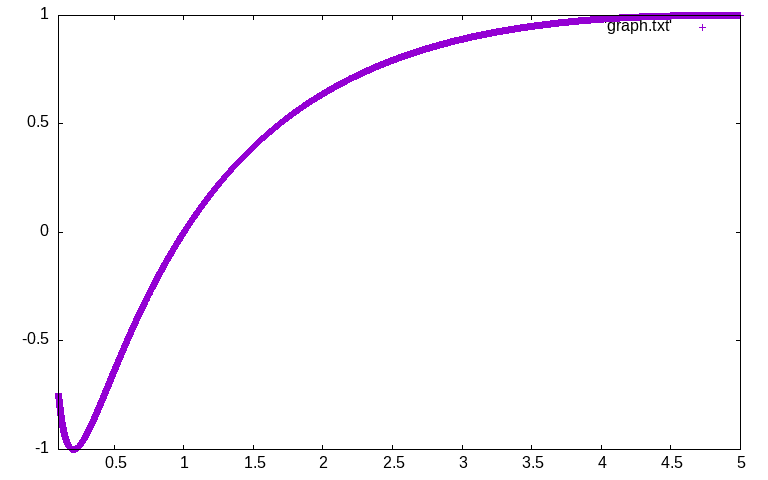
\includegraphics{./graph.png} 


\end{document}
